\documentclass[../Main.tex]{subfiles}
\begin{document}
\chapter{Data Analytics}

\intro{
    Data Analytics is the process of examining, cleaning, transforming, and 
    modelling data to extract useful insights, support decision-making, and 
    identify patterns. 
    It involves cleaning, transforming, and modelling data using statistical 
    analysis, machine learning, and data visualization to interpret complex 
    datasets. 
    Businesses, researchers, and organisations use data analytics to optimise 
    performance, predict trends, and drive strategic decisions.
}

\defn{Datenkompetenz (Data Literacy)}{
Umfasst die Fähigkeiten, Daten auf kritische Art und Weise zu sammeln, zu 
managen, zu bewerten und anzuwenden.

Grundlegende Fragen:
    \begin{enumerate}
        \item Was will ich mit Daten machen?
        \item Was kann ich mit Daten machen?
        \item Was darf ich mit Daten machen?
        \item Was soll ich mit Daten machn?
    \end{enumerate}
}

\section{Datentypen und Skalenniveaus}
Die Bestimmung der Datenmerkmale ermöglicht es erst, Daten zu 
organisieren, zu analysieren und schliesslich zu nutzen.
Das führt zu Skalenniveaus (Attributs-Merkmals-Levels, en: "Levels of 
measurement" or "Scales of measure")

\begin{figure}[H]
    \centering
    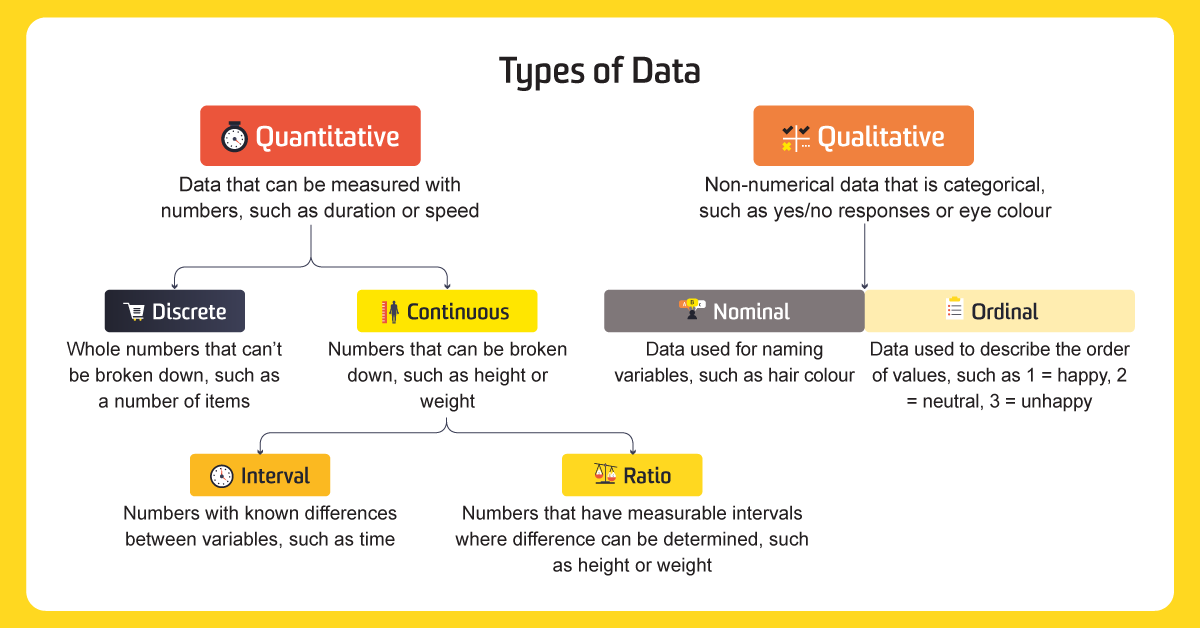
\includegraphics[width=0.75\linewidth]{Images/datentypen.png}
    \caption{Datentypen}
\end{figure}


\begin{multicols}{2}
    \defn{Qualitative Daten}{
        \begin{itemize}
            \item Beziehen sich auf Informationen die nicht gemessen werden
            \item In der Regel beschreibend also in Textform (können auch numerisch codiert sein).
        \end{itemize}
    }
    \defn{Quantitative Daten}{
        \begin{itemize}
            \item Werden verwendet, um Informationen zu definieren, die gezählt werden können. 
            \item Sind numerisch.
        \end{itemize}
    }
\end{multicols}

\defn{NOIR}{
    \begin{itemize}
        \item Nominalskala
        \item Ordinalskala
        \item Intervallskala
        \item Verhältnisskala (Ratio)
    \end{itemize}
}

\begin{figure}[H]
    \centering
    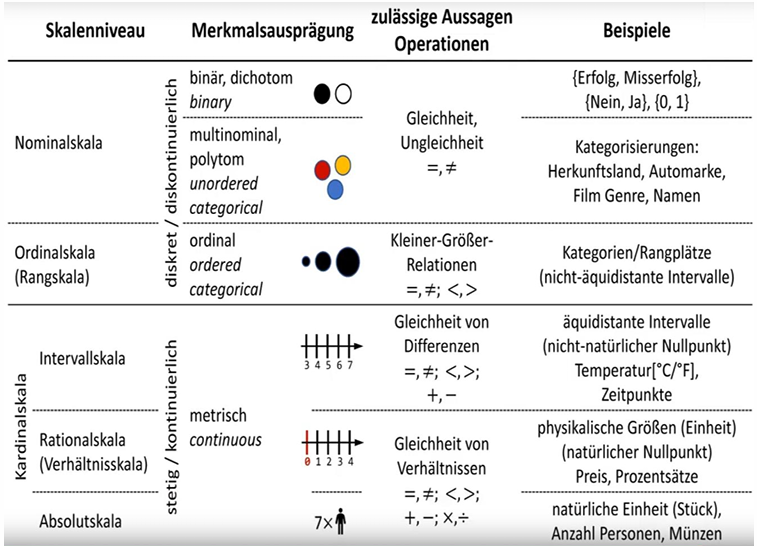
\includegraphics[width=0.75\linewidth]{Images/noir.png}
    \caption{NOIR}
\end{figure}

\section{Business Intelligence (BI)}
Datenvisualisierungs- und –Publikation-Werkzeuge ist allgemeiner  
und auch kurz Business Intelligence-Werkzeug (BI Tools) genannt.
Früher sprach man auch von Decision Support Systems.

\begin{multicols}{2}
    \defn{BI Tools}{
        Sind Tools und Technologien, die Unternehmen einsetzen, um Daten zu sammeln, zu 
        analysieren und in aussagekräftige Erkenntnisse und Wissen umzuwandeln, das für 
        fundierte Geschäftsentscheidungen genutzt werden kann. Umfasst den Einsatz von 
        Analyse, Data Mining, Data Warehousing und Reporting.
    }
    \defn{Decision Support Systems (DSS)}{
        Sind computergestützte Informationssysteme mit Methoden, die Entscheidungsträgern 
        helfen, bessere und fundiertere Entscheidungen zu treffen (bezüglich Ist-Zustand, 
        zurückblickenden Analyse).

        Dabei gibt es verschiedene Ansätze:
        \begin{itemize}
            \item Datenbankansatz (inkl. Visualisierung)
            \item Data-Mining-Ansatz
            \item Informationsbeschaffungsansatz
        \end{itemize}
    }
    BI liefert die Daten und Erkenntnisse, die für die Entscheidungsfindung erforderlich sind, 
    während DSS die Werkzeuge und Methoden für diese Entscheidungen bereitstellt.
\end{multicols}

Die wohl verbreitetsten Produkte sind die kommerziellen Anwendungen:
\begin{itemize}
    \item Tableau
    \item Ms Power BI
\end{itemize}
Weitere Produkte:
\begin{itemize}
    \item Looker
    \item Apache Superset
    \item Oracle Analytics
    \item Datawrapper
\end{itemize}


\begin{figure}[H]
    \centering
    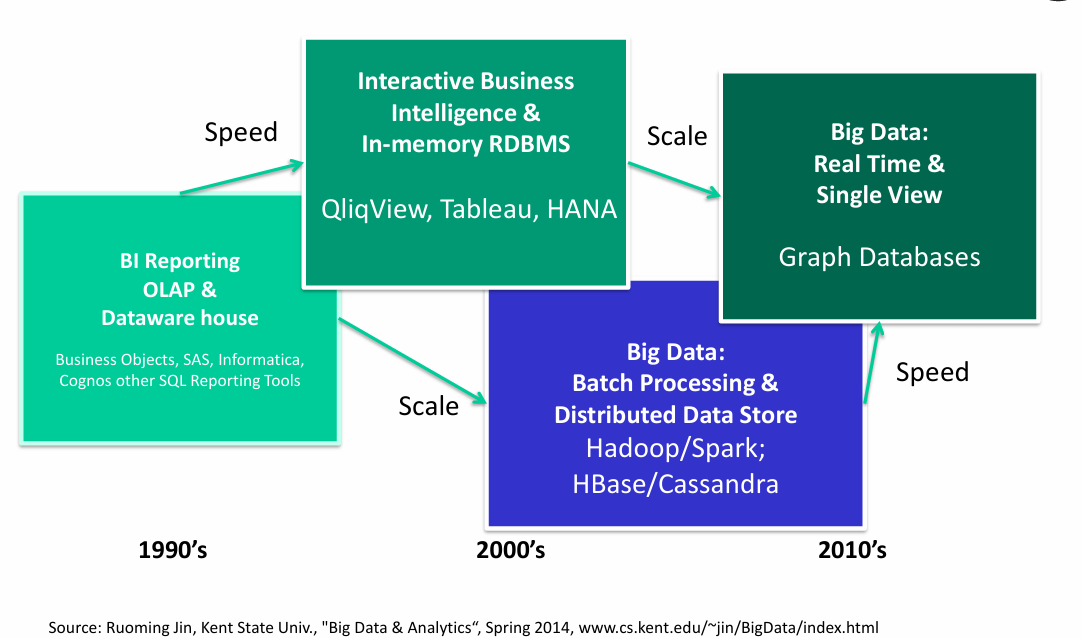
\includegraphics[width=0.75\linewidth]{Images/evolutionbi.png}
    \caption{Evolution of BI}
\end{figure}

\defn{7 Types of Quantitative Messages}{
    \begin{itemize}
        \item Nominal Comparison
        \item Time-Series
        \item Part-to-Whole
        \item Deviation
        \item Frequency distribution
        \item Correlation
    \end{itemize}
    Stephen Few
}

\begin{figure}[H]
    \centering
    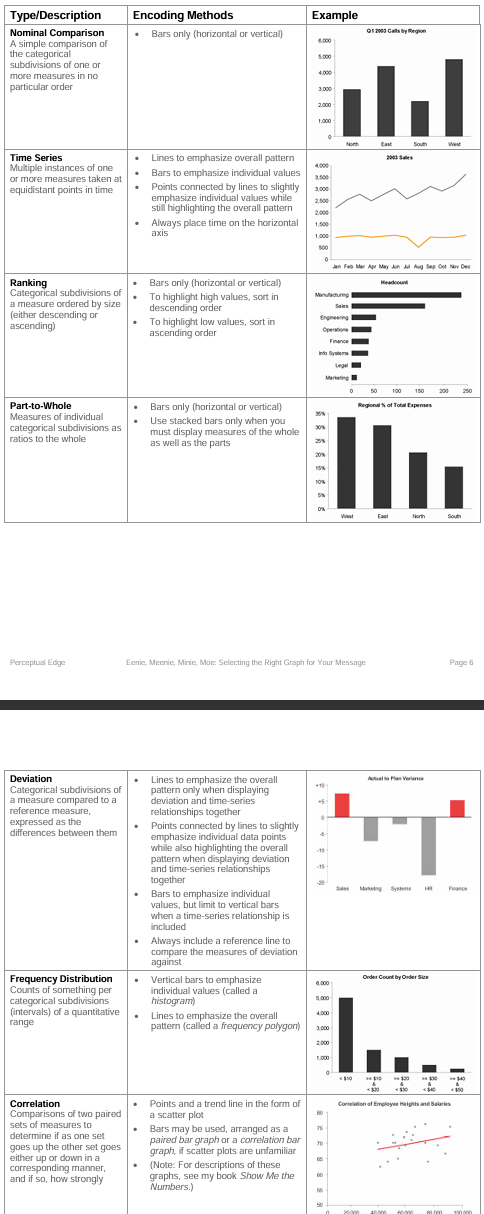
\includegraphics[width=0.5\linewidth]{Images/quantitative-messages.png}
    \caption{Quantitative Messages}
\end{figure}

\defn{Graphical Integrity by Tufte}{
    \begin{enumerate}
        \item The representation of numbers, as physically 
        measured on the surface of the graph itself, 
        should be directly proportional to the 
        numerical quantities represented.
        \item Clear, detailed and thorough labeling should 
        be used to defeat graphical distortion and 
        ambiguity. Write out explanations of the data 
        on the graph itself. Label important events in 
        the data.
        \item Show data variation, not design variation.
        \item In time-series displays of money, 
        deflated and standardized units of 
        monetary measurement are nearly 
        always better than nominal units.
        ("Deflating" means adjusting for inflation,
        so the values reflect purchasing power rather
        than just raw monetary amounts.)
        \item  The number of information carrying 
        (variable) dimensions depicted 
        should not exceed the number of 
        dimensions in the data.
        Graphics must not quote data out of context.
    \end{enumerate}
}

\defn{Data Ink Principles by Tufte}{
    \begin{enumerate}
        \item Above all else show data.
        \item Maximize the data-ink ratio.
        \item Erase non-data-ink.
        \item Erase redundant data-ink.
        \item Revise and edit
    \end{enumerate}
    The data-ink ratio is calculated by 1 minus the proportion of the graph 
    that can be erased without loss of data-information.
}

\begin{figure}[H]
    \centering
    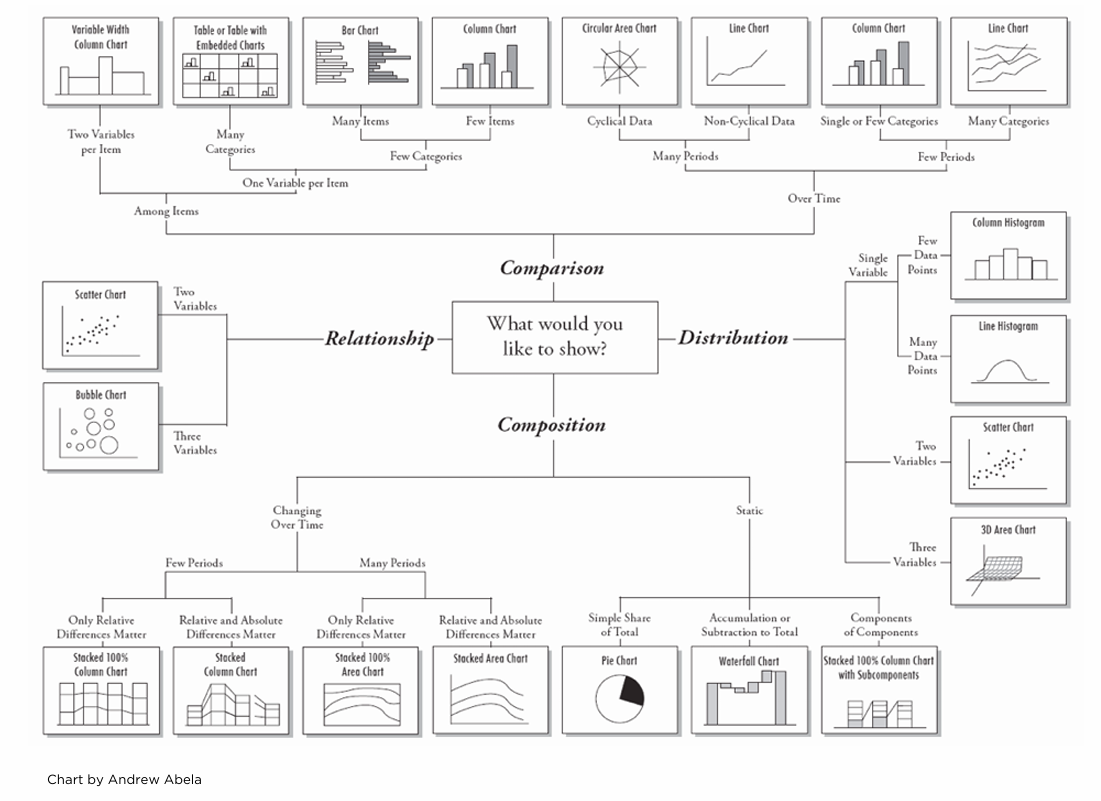
\includegraphics[width=1\linewidth]{Images/visualization-guideline.png}
    \caption{Visualization Guideline by Abela}
\end{figure}

\href{https://en.wikipedia.org/wiki/Visual_variable}{Visual Variable (Wikipedia)}


\section{OLAP}

\defn{Online Transaction Processing (OLTP)}{
    Zum Beispiel Flugbuchungssysteme.
    Charakterisierung:
    \begin{itemize}
        \item Hohe paralellität
        \item Viele kurze Transaktionen
        \item Transaktionen bearbeiten kleines Datenvolumen
        \item Mission-Critical
        \item Hohe Verfügbarkeit
        \item Normalisierte Relationen
        \item Wenige Indexe
    \end{itemize}
}

\defn{OLAP}{
    Überbegriff für Technologien, Methoden und Tools zur Ad-hoc-Analyse 
    multidimensionaler Informationen.
    Die Daten werden nach unterschiedlichsten (ad-hoc) Kriterien 
    ausgewertet.
}

\begin{figure}[H]
    \centering
    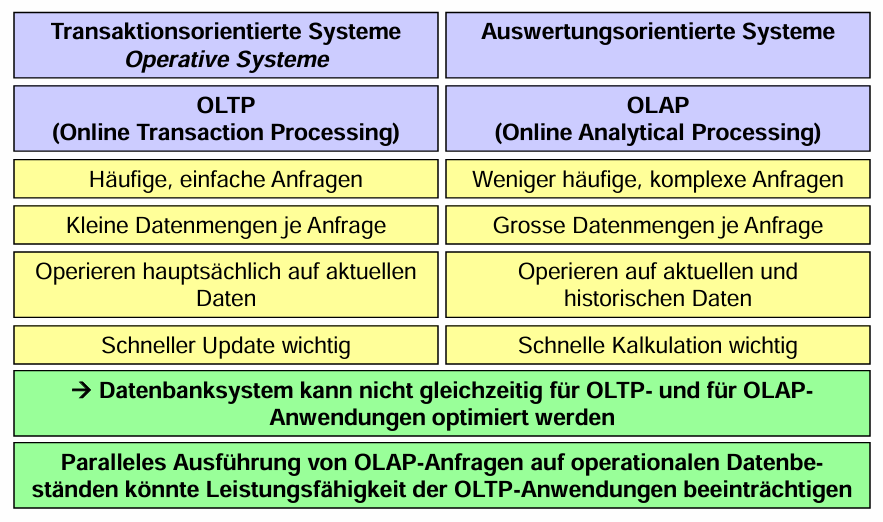
\includegraphics[width=1\linewidth]{Images/oltp-olap.png}
    \caption{OLTP vs OLAP}
\end{figure}


\begin{figure}[H]
    \centering
    \includegraphics[width=1\linewidth]{Images/olap-übersicht.png}
    \caption{OLAP Übersicht}
\end{figure}

\defn{Data Warehouse}{
    Ein Data Warehouse ist ein Datenbanksystem (für OLAP
    Anwendungen), in dem die entscheidungsrelevanten Daten eines 
    Unternehmens in konsolidierter Form gesammelt werden, um sie für 
    (zeitbasierte) Auswertungen zugänglich zu machen.
}

\begin{figure}[H]
    \centering
    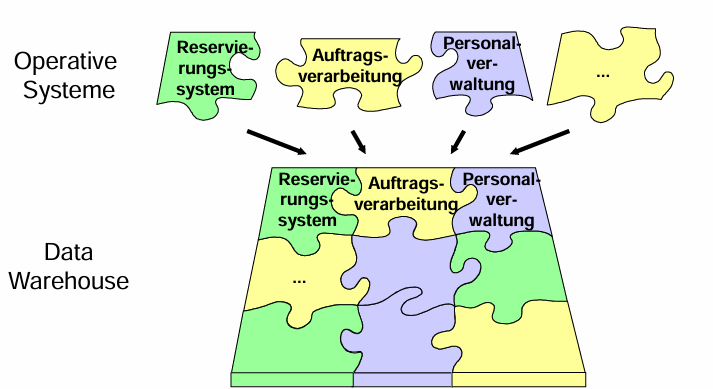
\includegraphics[width=1\linewidth]{Images/data-warehouse.png}
    \caption{OLTP vs OLAP}
\end{figure}

\defn{ETL - Extract-Transform-Load}{
    \begin{itemize}
        \item Aufbereitung von Daten aus heterogenen Quellen
        \item Laden ins Data-Warehouse
    \end{itemize}
}

\section{Relationale Data Warehouses}

\begin{figure}[H]
    \centering
    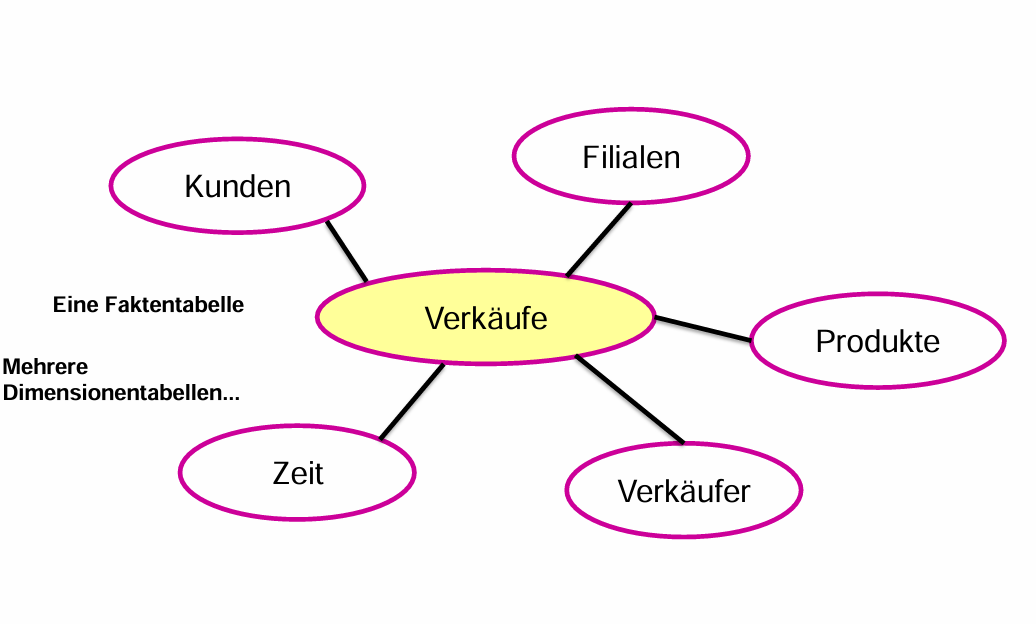
\includegraphics[width=0.75\linewidth]{Images/sternschema.png}
    \caption{Sternschema}
\end{figure}


\begin{figure}[H]
    \centering
    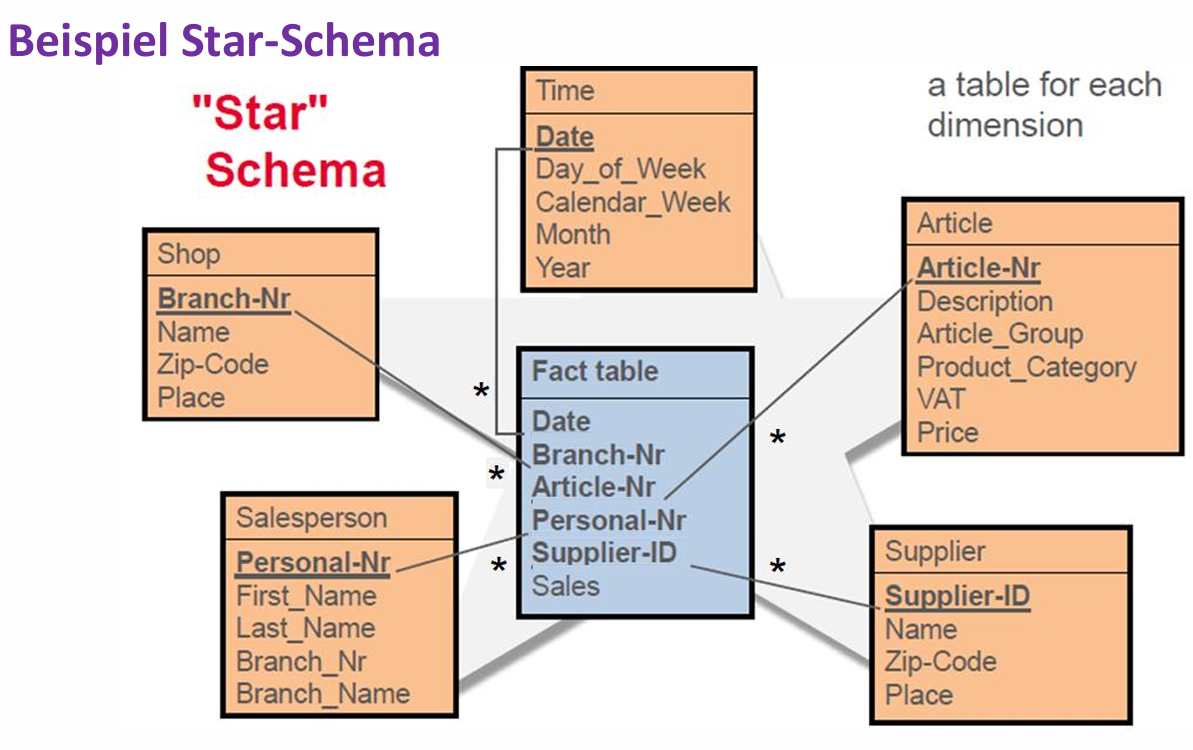
\includegraphics[width=0.75\linewidth]{Images/sternschema-beispiel.png}
    \caption{Beispiel einer Umsetzung des Sternschemas. Die Faktentabelle setzt sich ausschliesslich aus Foreign-Keys zusammen.}
\end{figure}

\defn{Sternschema}{
    Die Faktentabelle ist normalisiert und typischerweise sehr gross bis mehrere Mio Tuples,
    sie beinhaltet Bewegungsdaten mit weiteren Attributen, die Referenzen/FKs auf Dimensionstabellen sind.
    Die Dimensionstabellen beschreiben die Fakten in der Faktentabelle und sind
    oft nicht normalisiert und klein bis mittelgross (etwa 1'000).
    In der Regel werden Queries über 1-stufige Joins zwischen Fakten und verknüpften Dimensionen getätigt.
}

\begin{figure}[H]
    \centering
    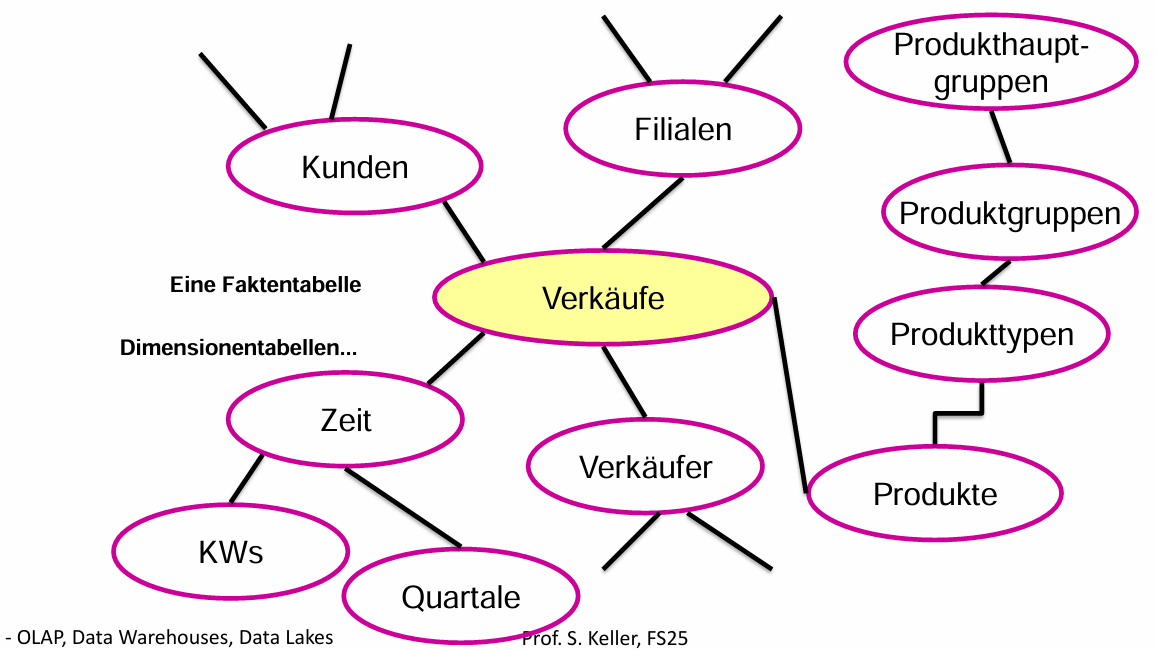
\includegraphics[width=0.75\linewidth]{Images/schneflockenschema.png}
    \caption{Die Normalisierung der Dimensionstabellen führt zum Schneeflocken-Schema.}
\end{figure}

\defn{Schneeflocken-Schema}{
    Normalisierung der Dimensionen im Sternschema führt zum Schneeflocken-Schema.
    Pro Hierarchielevel kann in der Regel mit einer Tabelle gerechnet werden.
    Das bedeutet Abfragen über Joins werden kompliziert, daher hat sich das Schema eher nicht durchgesetzt.
}

\subsection{Data-Warehouse Design Grundsätze}
auch "Dimensional Modeling" genannt.
\begin{itemize}
    \item Faktentabellen enthalten nur numerische Werte und Fremdschlpssel
    \item Faktentabellen sollten so granular wie möglich aufgebaut sein. (einfacher zum Aggregieren)
    \item Dimensionstabellen haben in der Regel einen Surrogat-Schlüssel
    \item Granularität der Zeit-Dimension kann nicht kleiner sein, als die Auflösung der Zeit im operativen System
    \item "Conformed Dimensions" haben für alle möglichen Fact-Tables eine einheitliche Bedeutung
    \item Hierarchien in Dimensionen sind möglichst als funktionale Abhängigkeit zwischen den Attributen einer
    flaachen Dimensionstabelle oder als Fremdschlüsselbeziehung zwischen Dimensionstabellen zu konzipieren.
\end{itemize}

\subsection{Fakt-Tabellen}
\begin{description}
    \item[Transaction Fact Table] Ereignis, dass zu einem bestimmten Zeitpunkt geschah
    \item[Periodic Snapshot] kumulative Grösse einer Kennzahl gemessen in regelmässigen Intervallen
    \item[Accumulating Snapshot] Eintrag beschreibt eine Business-Transaktion aus mehreren Schritten zu unterschiedlichen Zeitpunkten   
\end{description}

\subsection{Spezielle Dimensionen}
\begin{description}
    \item[Degenerate Dimension] Identifizieren eine Transaktion (z.B Order Header)
    \item[Role Playing Dimension] Dimension wird von Fact-Table mehrfach unterschiedlich bedeutend referenziert
    \item[Junk Dimensions] Korrelierte Indikationen und Flags 
\end{description}

\defn{Slowly Changing Dimensions}{
    "Veränderungen treten unerwartet, sporadisch und weitaus seltener auf als Messungen in Faktentabellen"
    \begin{description}
        \item[Typ 1] Keine Historisierung (Overwrite)
        \item[Typ 2] Historisierung mittels neuem Zeilen-Eintrag und Attribute PK-BK valid-from und valid-to
        \item[Typ 3 bis 6] Weitere Historisierung durch zusätzliche Zeit-Attribute oder Tabellen  
    \end{description}
}


\begin{figure}[H]
    \centering
    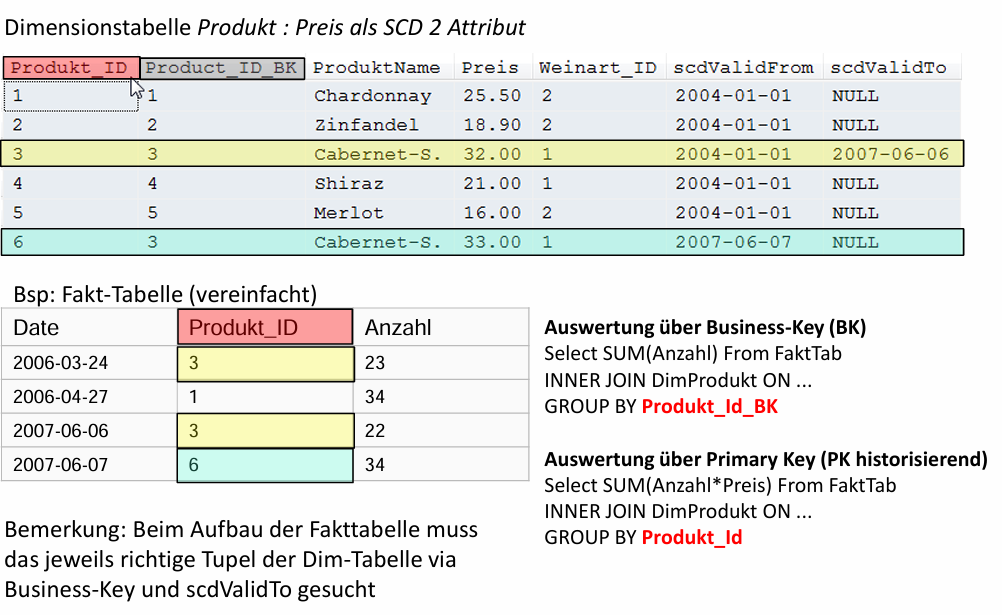
\includegraphics[width=0.75\linewidth]{Images/scd-typ-2.png}
    \caption{SCD Typ 2}
\end{figure}

Typ 2 SCD wird z.B von MSSQL und Azure SQL unterstütz unter dem Namen "system-versioned temporal tables".

\section{Aggregationsfunktionen und Pivot}

\defn{GROUP BY ROLLUP}{
    Ähnlich zu GROUPBY mit Vernubderzbg des Detaukkuerzbgsgrades,
    Bei ROLLUP(A,B) werden Daten zuerst nach A und dann nach B aggregiert und anschliessen noch ein Total beigefügt.
}

\begin{figure}[H]
    \centering
    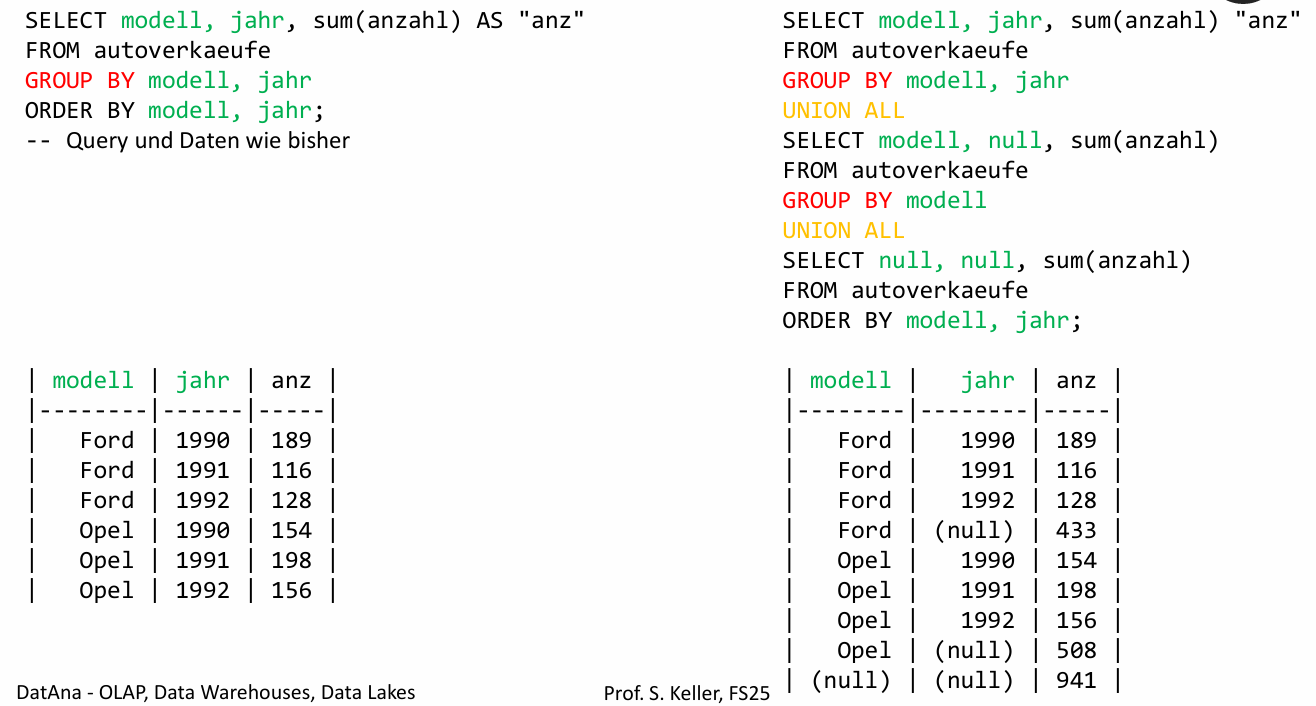
\includegraphics[width=0.75\linewidth]{Images/rollup.png}
    \caption{ROLLUP Befehl}
\end{figure}

\defn{GROUP BY CUBE}{
    Ähnlich wie der ROLLUP-Befehl fügt jedoch jedes Zwischentotal dazu.
    Erfordert für die Generierung die Potenzmenge der zu aggregierenden Spalten.
}

\begin{figure}[H]
    \centering
    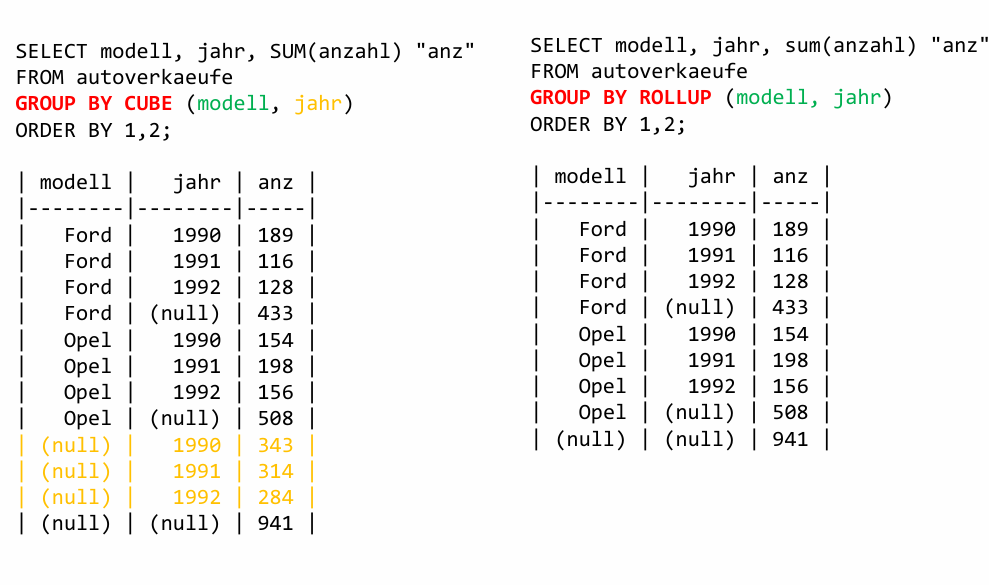
\includegraphics[width=0.75\linewidth]{Images/cube.png}
    \caption{CUBE Befehl}
\end{figure}

\begin{figure}[H]
    \centering
    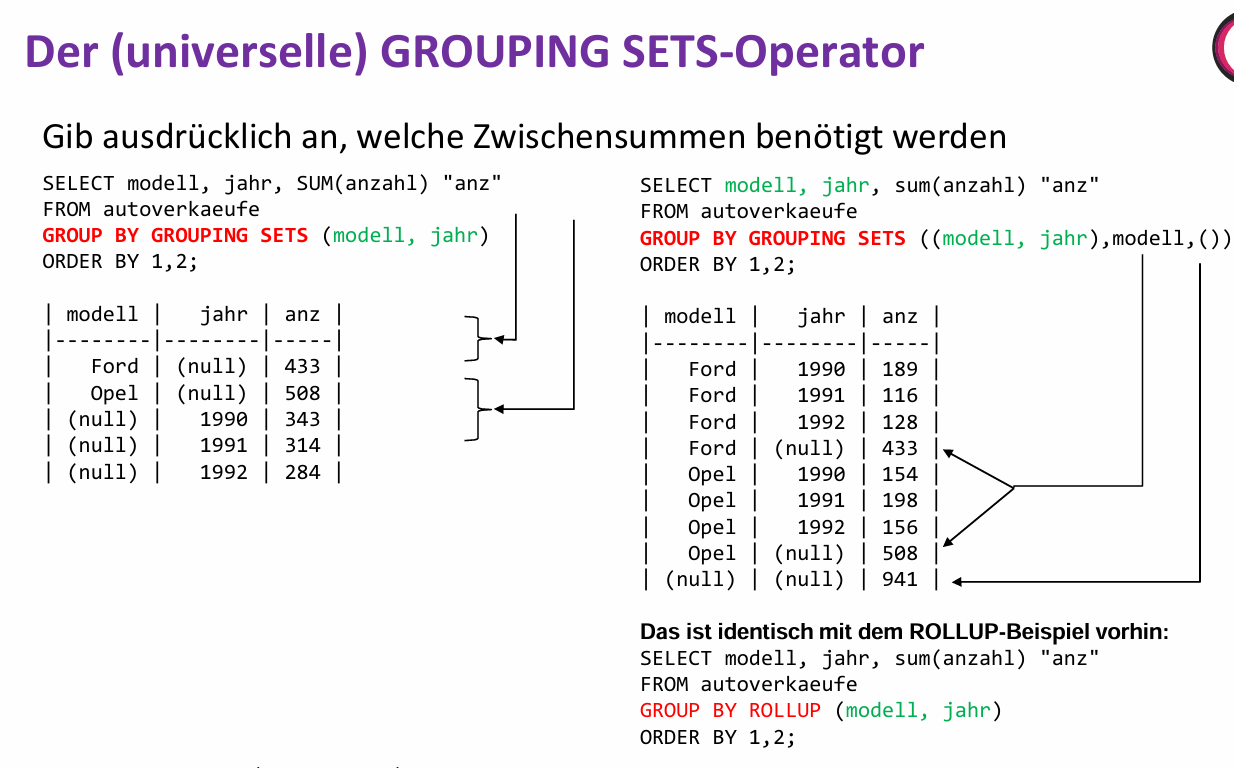
\includegraphics[width=1\linewidth]{Images/groupingset.png}
    \caption{Grouping Sets Operator; Dieser kann generell anstelle von ROLLUP und CUBE eingesetzt werden
    Zwischenresultate müssen explizit verlangt werden.}
\end{figure}

\defn{Pivot-Tabelle}{
    Tabellenspalten werden aggregiert und transponiert, dies nennt man Pivotieren (drehen).
    Es wird typischerweise in Statistik und Marktforschung verwendet zusammen mit Aggregationsfunktionen.
    Pivot- und Kreuz-Tabellen sind praktisch synonyme.

    Bei PSQL nicht integriert aber kann statisch via "crosstab" oder dynamisch über "tablefunc" erstellt werden.
}

\begin{figure}[H]
    \centering
    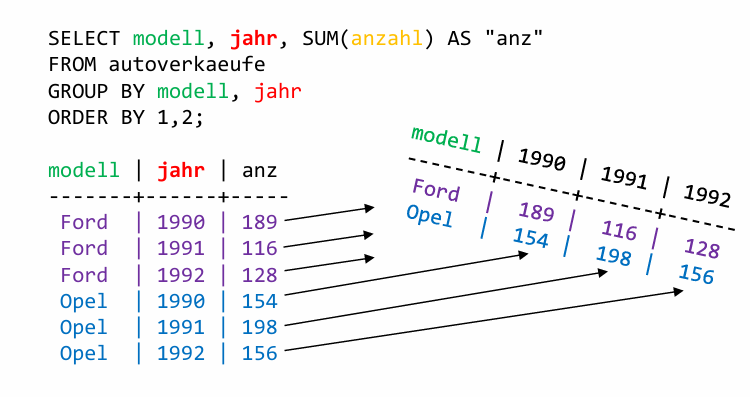
\includegraphics[width=0.5\linewidth]{Images/pivot.png}
    \caption{Pivot}
\end{figure}

\begin{figure}[H]
    \centering
    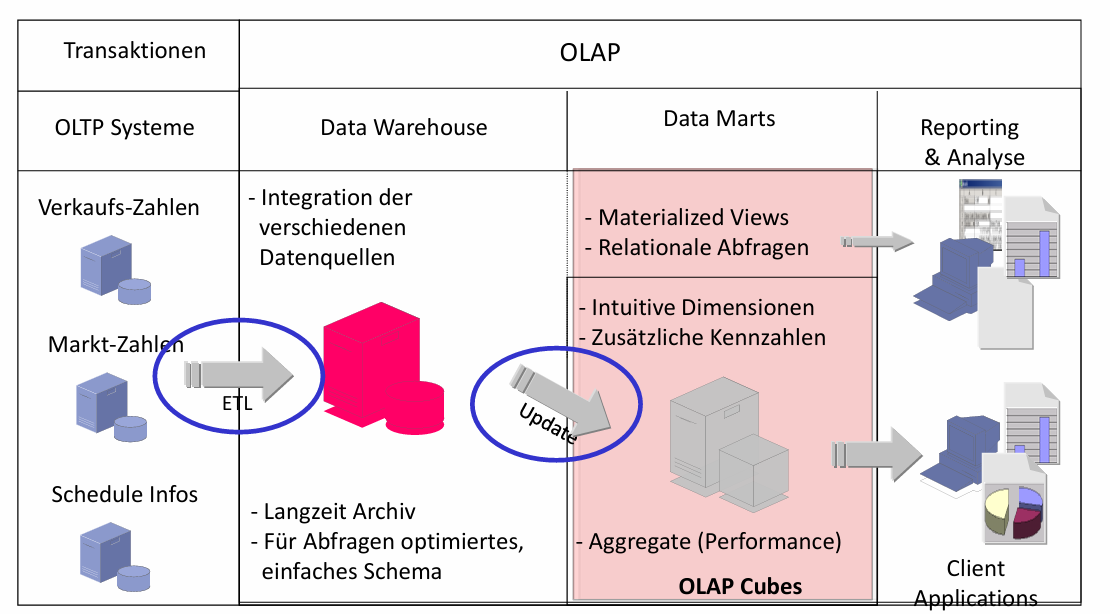
\includegraphics[width=0.5\linewidth]{Images/datamarts.png}
    \caption{Data Marts: }
\end{figure}

\defn{Data Marts}{
    Für den Zugriff auf Teilmenge eines Data Warehouses für bestimmte Subeinheiten eines Systems.
    Data Marts sind kleiner und flexibler als das Datawarehouse.
    Sie können strukturierte oder unstrukturierte Daten schnell und durch optimierte Abfragen (Vorberechnung \& Speicherung)
    bereitstellen. (z.B Materialized View, Cube-Datastructures)

    Wenn weitere Optimierung nötig ist, kann z.B MDX von Microsoft benutzt werden, welche Data-Cubes als
    Datenstrukturen und Abfragesprache zur Verfügung stellt.
}

\defn{Data Lake}{
    Speichersystem für strukturierte und unstrukturierte Daten in ihrem ursprünglichen Format.
}

\begin{figure}[H]
    \centering
    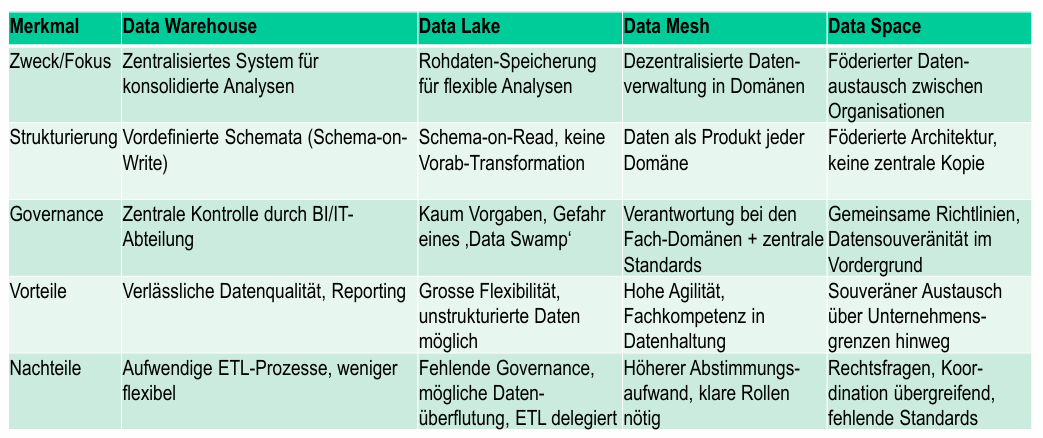
\includegraphics[width=0.72\linewidth]{Images/da-begriffe.png}
\end{figure}

\section{Spatial Data}
\defn{EVAP}{
    \begin{itemize}
        \item Erfassung
            \begin{itemize}
                \item GPS (Outdoor)
                \item DGPS (Outdoor)
                \item 3D-Scanner (Kinect)
                \item WLAN
                \item Bluetooth
                \item Kamera (SLAM)
            \end{itemize}
        \item Verwaltung (Speicherung)
            \begin{itemize}
                \item Kommerziell: ArcGIS, Oracle, MSSQL, MongoDB
                \item Open Source: PostGreSQL, MySQL, DuckDB
                \item Geodatentypen, Funktionen, Indexe
            \end{itemize}
        \item Analyse
        \item Präsentation Darstellung
        \end{itemize}
}

\begin{figure}[H]
    \centering
    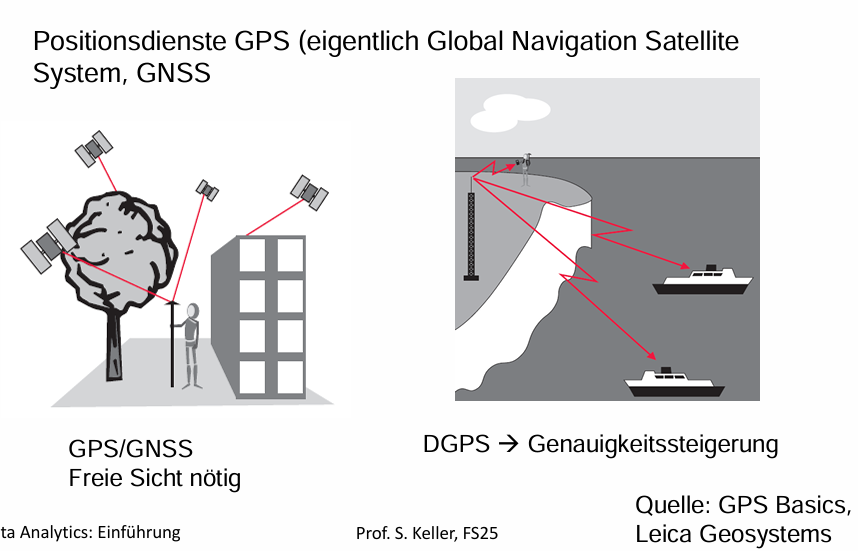
\includegraphics[width=0.75\linewidth]{Images/evap-eingabe.png}
    \caption{EVAP: Eingabe / Erfassung}
\end{figure}

\defn{Geodaten (Geospatial Data)}{
    Sind allgemein Daten mit Raumbezug
    \begin{itemize}
        \item Geografische Namen
        \item Adressen
        \item Codes
        \item Punkte, Linien, Flächen, Pixel/Voxel
    \end{itemize}
    Geodaten weisen eine komplexe Datenstruktur mit vielen Formaten auf.
    Sie sind:
    \begin{itemize}
        \item komplexe Konsistenzbedingungen
        \item Grosser Erfassungsaufwand
        \item Grosse Datenmengen
        \item Viele Metadaten
            \begin{itemize}
                \item Koordinaten Referenzsystem
                \item Auflösung
                \item Qualität
            \end{itemize}
    \end{itemize}
}

\subsection{Raumbezug - Projektion}
Eine 2D Abbildung unseres 3D Raumes ist schwierig.
Der Modellierungsprozess erfordert abstraktion, welcher zu Informationsverlust führen kann.

\begin{figure}[H]
    \centering
    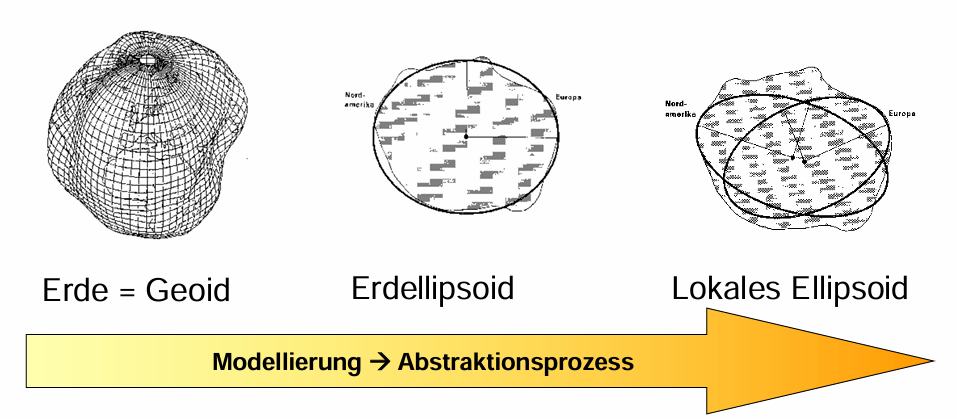
\includegraphics[width=0.75\linewidth]{Images/raumbezug.png}
    \caption{Raumbezug - Projektion}
\end{figure}
Längengrad/Breitengrad sind ein "geozentrischer 
Vektor". Karten und Bildschirme sind jedoch 
"eben/flach".
\\\\
Eine Projektion bildet das Ellipsoid auf eine Fläche 
ab, d.h. auf kartesische Koordinaten: der Nordwert 
(Mathe Y) und der Ostwert (Mathe X) und stehen 
rechtwinklig zueinander.
\\\\
Koordinatensysteme inkl. Projektionen erhalten 
eine Abkürzung, z.B. CHLV95 (Schweizerische 
Landesvermessung 1995) oder WGS84 (World 
Geodetic System) und einen Code

\defn{Bekannte Codes}{
    \begin{itemize}
        \item WGS84 - EPSG-Code:4326 ("GPS-Koordinaten")
            \begin{itemize}
                \item geozentrisch, geografisch, Grad
                \item Beiten/Längengrad (lat/lon N/E)
            \end{itemize}
        \item Web Mercator - EPSG-Code 3857 ("Schulwandkarte")
            \begin{itemize}
                \item kartesisch (=eben), metrisch
            \end{itemize}
        \item CHLV95 - EPSG-Code 2056 ("Schweizer Koordinatensystem")
            \begin{itemize}
                \item Landvermessung CH neu, kartesisch-metrisch
                \item 7-stellige Koordinaten
            \end{itemize}
    \end{itemize}
    Die National Geospatial-Intelligence Agency der USA empfiehlt WGS 84 (EPSG:4326). Sie rät von 
    Web Mercator (EPSG:3857) für militärische und nachrichtendienstliche Zwecke ab, da es 
    Probleme mit der Positionsgenauigkeit gibt, insbesondere in hohen Breitengraden.
}

\begin{figure}[H]
    \centering
    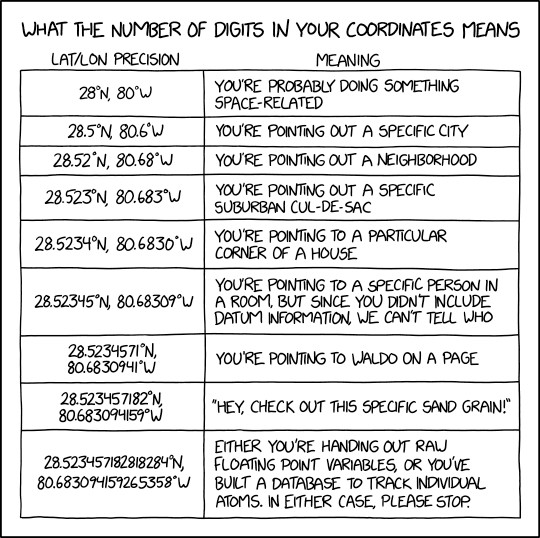
\includegraphics[width=0.5\linewidth]{Images/coordinate_precision.png}
    \caption{Koordinatenpräzision}
\end{figure}

\subsection{GIS Architecture}
\begin{itemize}
    \item  Produktpalette mit ArcGIS Pro und ArcGIS Online als bekannteste Produkte
    \item  QGIS Projekt (Open Source GPL)
\end{itemize}

\begin{figure}[H]
    \centering
    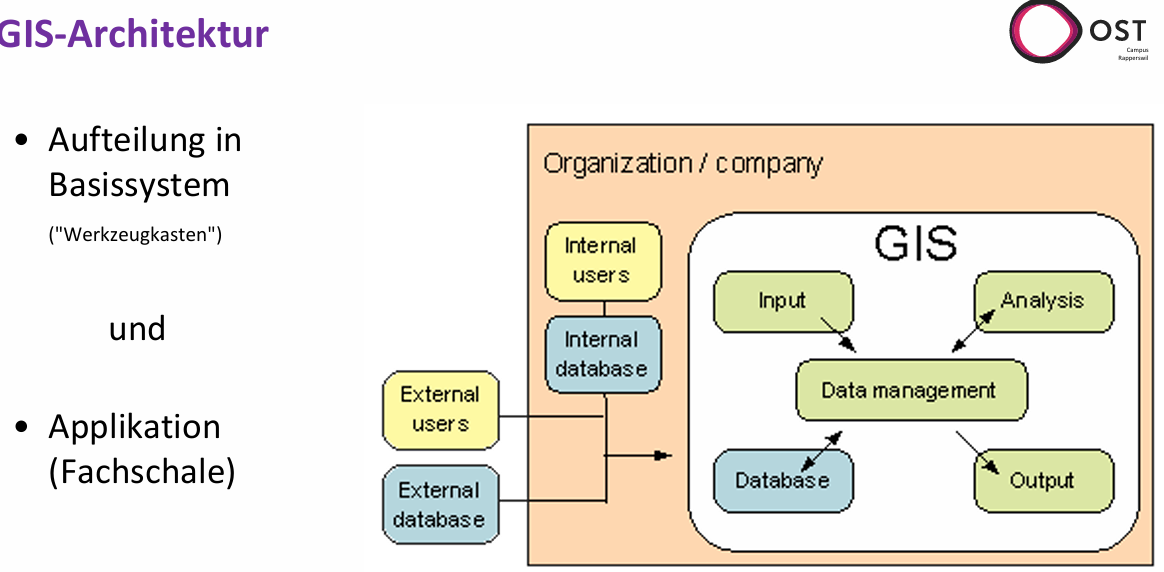
\includegraphics[width=0.5\linewidth]{Images/gis-architektur.png}
    \caption{GIS: Generelle Architektur}
\end{figure}
\begin{figure}[H]
    \centering
    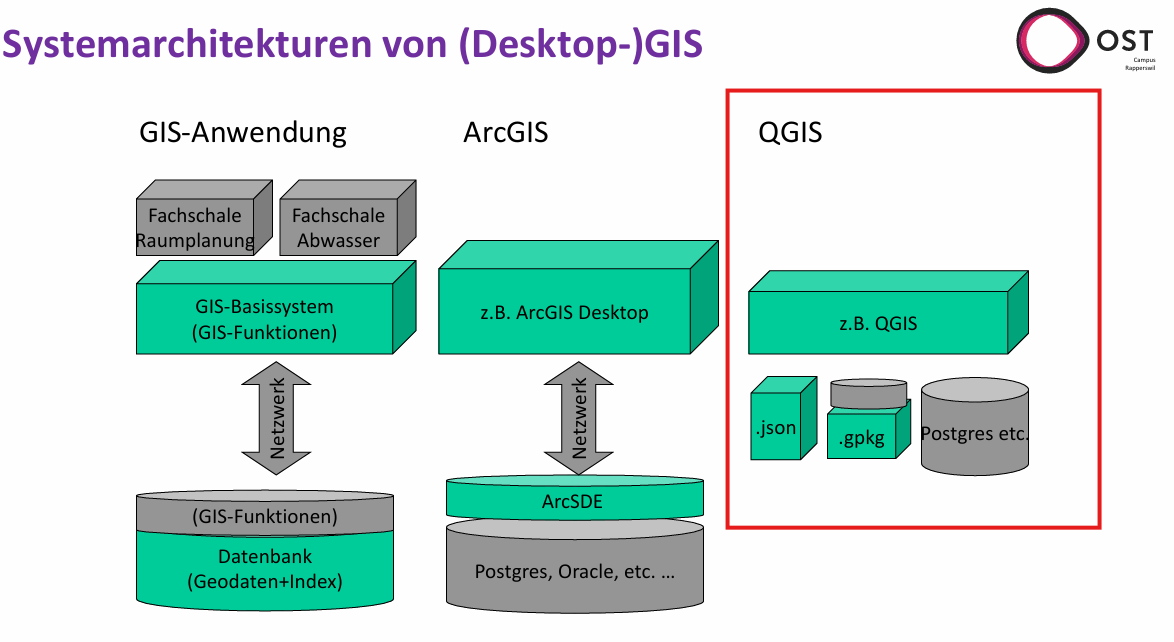
\includegraphics[width=0.5\linewidth]{Images/gis-architekturen.png}
    \caption{GIS: Produkt Architektur}
\end{figure}

\subsubsection{Web-Apps}
\begin{figure}[H]
    \centering
    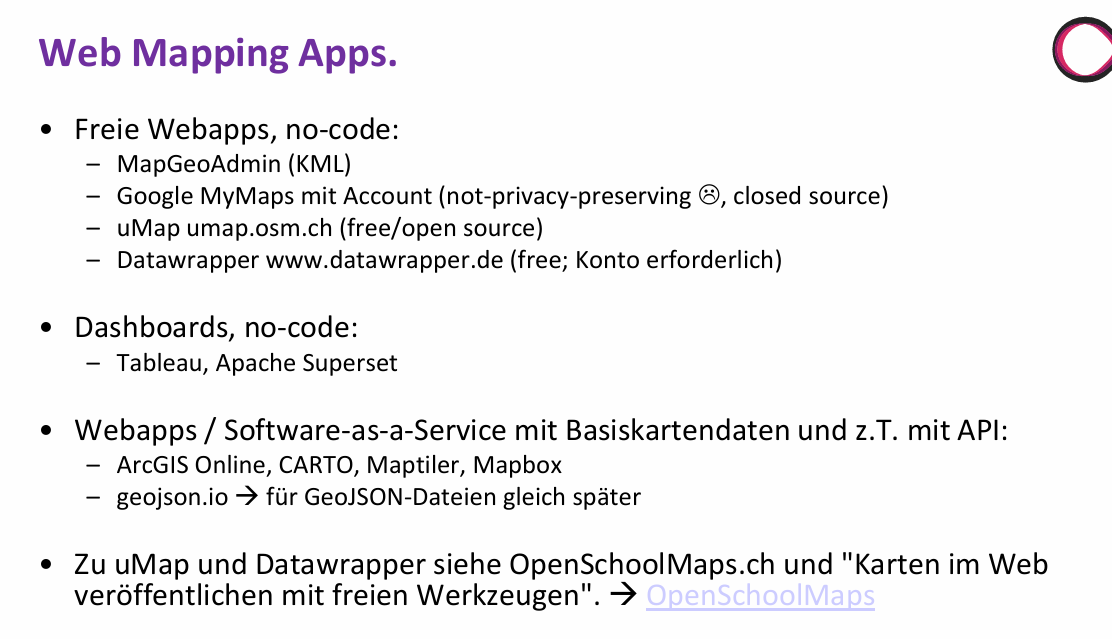
\includegraphics[width=0.75\linewidth]{Images/gis-webapps.png}
    \caption{GIS: Webapps}
\end{figure}

\subsubsection{Geovisualisierung für Data Engineers}
\begin{figure}[H]
    \centering
    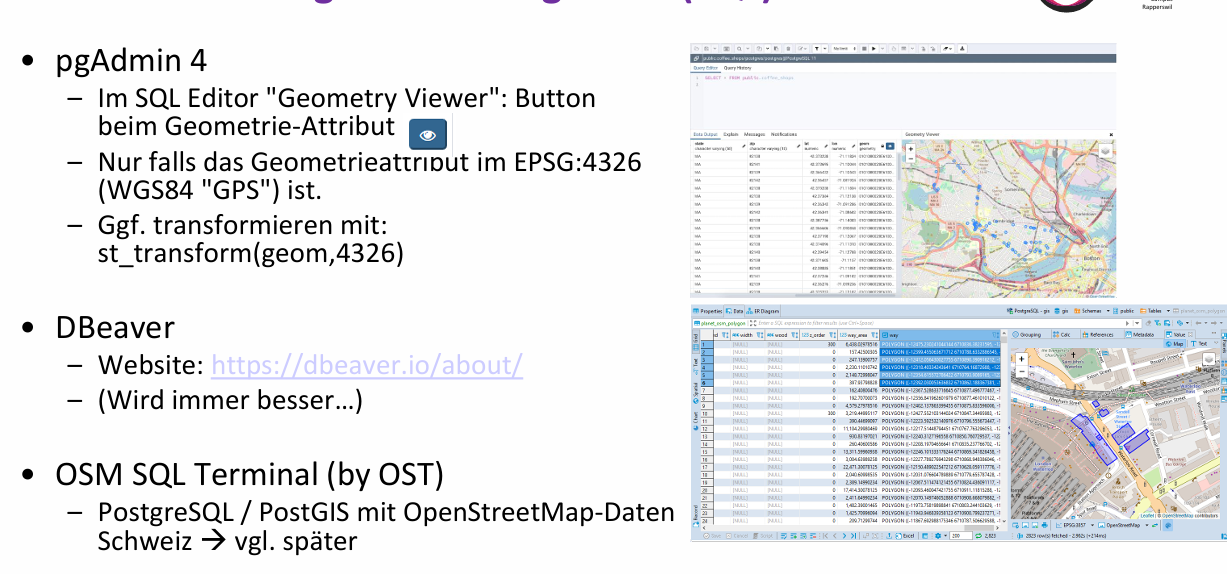
\includegraphics[width=0.75\linewidth]{Images/geovisualisierung-data-eng.png}
    \caption{Geovisualisierung für Data Engineers}
\end{figure}

\subsection{Prinzipien von GIS Verarbeitung}
\defn{Ebenenprinzip}{
    Informationen werden in Ebenen übereinander geschichtet.
    Koordination ermöglichen einen vertikalen Lagenvergleich.
    Die Stärke von GIS ist durch Kombination unabhängiger Daten neue Informationen abzuleiten.
}
\begin{figure}[H]
    \centering
    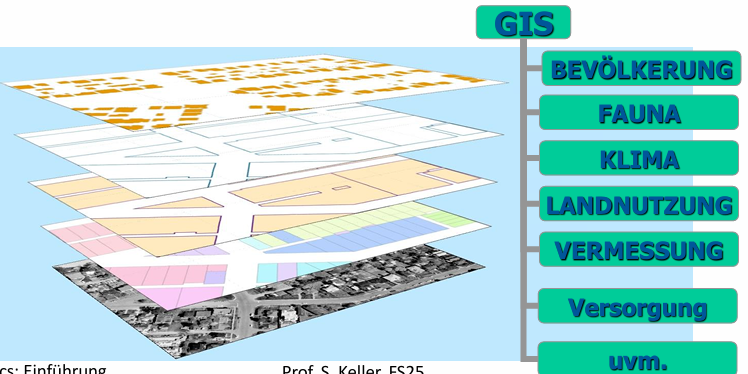
\includegraphics[width=0.5\linewidth]{Images/gis-layers.png}
    \caption{Layerprinzip}
\end{figure}

\defn{Universelle Fremdschlüssel (Raumbezug)}{
    Der Razmbezug wird als gemeinsamen Nenner aller Objekte herangezogen.
    Koordinaten sttelllen einen grundsätzlich neuen Beziehungstyp dar,
    der Kombinationen z.b via räumlichen Joins erlaubt.
}

\defn{Modellierung / Repräsentation}{
    \begin{itemize}
        \item Diskret (Räumlich begrenzt), z.B Gebäude
        \item Kontinuierlich (Felder), z.B Luftdruck
    \end{itemize}
    Diese werden codiert:
    \begin{itemize}
        \item Vektorbasiert (Vektordaten)
            \begin{itemize}
                \item Geometrische Datentypen Punktkoordinaten, Linien und Flächen
                \item Einzeln ansprechbar, gruppierbar, skalierbar, "berechenbarer"
            \end{itemize}
        \item Rasterbasiert (Rasterdaten, z.B Bilder)
            \begin{itemize}
                \item zusammengehörige Menge von (Farb-)Pixeln, die einen Raumbezug haben (sie 
                sind sogenannt "geo-referenziert")
                \item Erfasst durch CCD/CMOS-Sensoren in Scanner und Kameras; z.B. GeoTIFF-Format
                \item Schneller in Darstellung als Vektoren, billiger in der Herstellung
            \end{itemize}
    \end{itemize}
}

\begin{figure}[H]
    \centering
    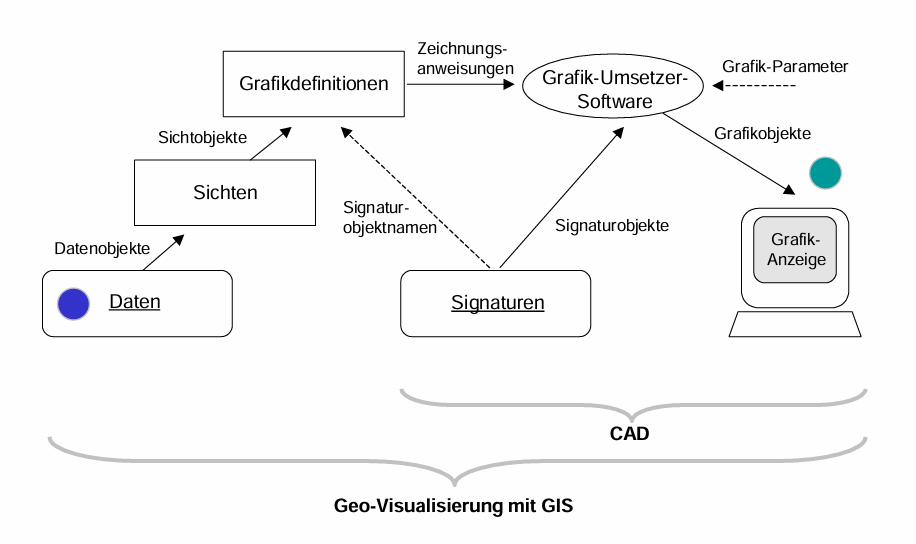
\includegraphics[width=0.5\linewidth]{Images/geodaten-zu-grafik.png}
    \caption{Geodaten zu Grafik}
\end{figure}

\subsubsection{Geodaten Vektor Formate}
\begin{itemize}
    \item GeoJSON
        \begin{itemize}
            \item Lesbar
        \end{itemize}
    \item GeoPackage
        \begin{itemize}
            \item Verbessertes Shapefile
            \item Erweiterung SQLite
            \item Binärformat
        \end{itemize}
    \item Shapefile
        \begin{itemize}
            \item Industrie Norm
            \item Binär
            \item 2 Abhängige Dateien (Geometrie (.shp) + Sachdaten (.dbf))
            \item Veraltet
        \end{itemize}
    \item DXF
        \begin{itemize}
            \item Reine Geometrie/CAD
            \item Keine Sachdaten
        \end{itemize}
    \item GeoParquet
        \begin{itemize}
            \item Erweiterung Parquet
            \item Spaltenorientiert
            \item Offenes Speicherformat für effiziente Komprimierung (\&schnelle Abfragen)
        \end{itemize}
    \item CSV
    \item SVG
\end{itemize}
Konvertierungsprogramme:
\begin{itemize}
    \item https://geoconverter.infs.ch/
    \item https://mygeodata.cloud/converter/
\end{itemize}

\subsubsection{Geodaten Raster Formate}
\begin{itemize}
    \item PDF
    \item PNG, JPG
    \item TIFF, GeoTIFF
        \item Standard
\end{itemize}

\begin{figure}[H]
    \centering
    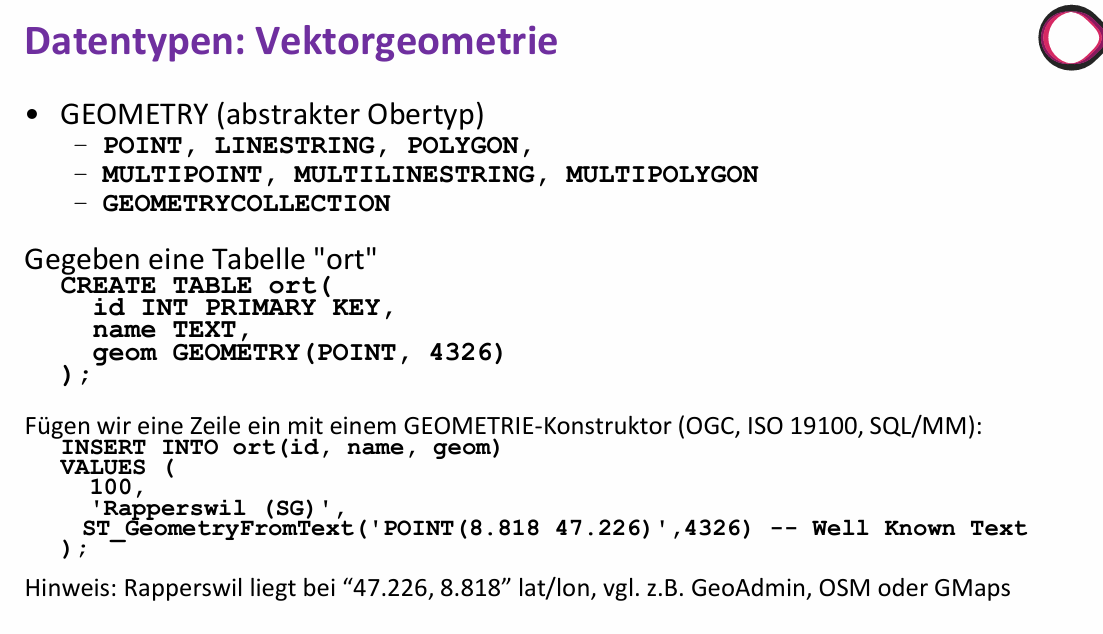
\includegraphics[width=0.75\linewidth]{Images/postgis-vektordatentypen.png}
    \caption{PostGIS Vektordatentypen}
\end{figure}

\begin{figure}[H]
    \centering
    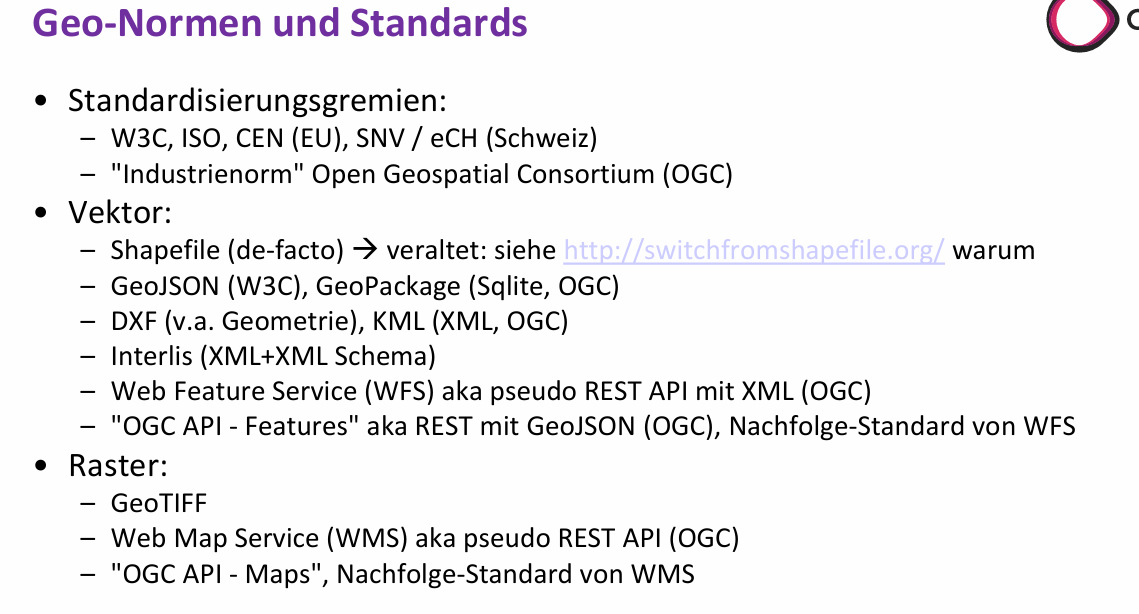
\includegraphics[width=0.75\linewidth]{Images/geonormen.png}
    \caption{Geo-Normen}
\end{figure}

\begin{lstlisting}[language=SQL]
    CREATE TABLE eisenbahn (
        id int4 PRIMARY KEY, 
        name TEXT,
        geom GEOMETRY('LINESTRING', 2056)
    );

    CREATE INDEX 
        in_eisenbahnen_the_geom
        ON eisenbahnen
        USING gist(geom);


    INSERT INTO uster(id, name, geom) VALUES (
        100,
        'Uster'
        ST_GeometryFromText('LINESTRING(8.81 47.22,8.81 47.22)',4326)  
    );

    SELECT id, name, ST_AsText(geom) FROM uster;

    CREATE TABLE beers (
        id GENERATED ALWAYS AS IDENTITY,
        name VARCHAR(60),
        price NUMERIC(10, 2),
        geom GEOMETRY('POINT', 4326)
        -- use usually a planar CRS not a geocentric
    );

    select name, price,
        round((price + 0.001 * ST_DistanceSphere(geom, 
            ST_GeometryFromText(
                'POINT(8.816511 47.223064)',4326)))::numeric, 2
            ) as net_price
    from beers order by net_price;
\end{lstlisting}

\subsection{PostGIS Queries}
\begin{lstlisting}[language=SQL]
-- Aufgabe 5.1: Distanzberechnung
-- => Im Lokalkoordinatensystem
SELECT ST_distance(
    (SELECT geom FROM orte 
        WHERE "name" = 'Bern' AND type = 'Medium City'),
    (SELECT geom FROM orte
        WHERE "name" = 'Zurich'AND type = 'Medium City'));
-- => basierend auf einer Kugel
SELECT ST_distanceSphere(
    (SELECT ST_Transform(geom,4326) FROM orte
        WHERE "name" = 'Bern' AND type = 'Medium City'),
    (SELECT ST_Transform(geom,4326) FROM orte
        WHERE "name" = 'Zurich'AND type = 'Medium City')
    );
-- => basierend auf einem Bessel 1841 Ellipsoid.
SELECT ST_distanceSpheroid(
    (SELECT ST_Transform(geom,4326) FROM orte
        WHERE "name" = 'Bern' AND type = 'Medium City'),
    (SELECT ST_Transform(geom,4326) FROM orte
        WHERE "name" = 'Zurich'AND type = 'Medium City'),
    'SPHEROID["Bessel 1841",6377397.155,299.1528128]');


-- Aufgabe 5.2: Objektselektion mit angrenzenden Flaechen
-- Selektieren Sie alle Gemeinden,
-- die an die Gemeinde Rapperswil-Jona grenzen.
SELECT * FROM gemeinden
WHERE ST_Touches(
    geom, 
    (SELECT geom FROM gemeinden WHERE name = 'Rapperswil-Jona')
) 
ORDER BY name ASC;


-- Aufgabe 5.3: Objektselektion als Umkreissuche
-- Selektieren Sie alle Orte im Umkreis
-- von 10 km um die HSR (CH1903: 704472/231216)
SELECT name, geom 
FROM orte
WHERE ST_DWithin(geom, 
    ST_GeomFromText('POINT(704472 231216)', 21781),10000)
ORDER BY name ASC;


-- Aufgabe 5.4: Pufferzone
-- Selektieren Sie alle Orte, die in einer Pufferzone
-- von 2km um den Fluss Emme liegen.
SELECT name 
FROM orte
WHERE ST_Within(
    geom,
    (SELECT ST_Buffer(geom, 2000) FROM fluesse WHERE name = 'Emme')
)
ORDER BY name ASC;


-- Aufgabe 5.5. 
-- Schreiben Sie eine Query, die alle Gemeinden selektiert,
-- durch die der Fluss Emme fliesst. 
SELECT g.name 
FROM gemeinden g
WHERE ST_Intersects(geom, (SELECT geom FROM fluesse WHERE name = 'Emme'))
ORDER BY 1;
-- oder 
SELECT g.name 
FROM gemeinden g
JOIN fluesse f ON ST_Intersects(f.geom, g.geom)
WHERE f.name = 'Emme' 
ORDER BY 1;
    
\end{lstlisting}

\section{Big Data}
\defn{Big Data}{
    Zu "Big Data" gib es keine einheitliche Definition; wird häufig auch als 
    Sammelbegriff verwendet für (Real-Time-)Analyse massiver Datenmengen.

    Unterteilunge auch möglich:
    \begin{itemize}
        \item Small Data: Memory eines einzelnen Systemes
        \item Medium Data: Auf Disk eine Systems
        \item Big Data: Erfordert verteilte Systeme
    \end{itemize}

    Blogbeitrag von Jordan Tigani (*), Zusammenfassung:
    \begin{itemize}
        \item Meisten Daten <100GB
        \item Wenn doch, wahrscheinlich nicht alle auf einmal abgefragt
    \end{itemize}
    (*) "Big Data is Dead" (2023) by Jordan Tigani, DuckDB Maintainer (Open Source); 
    vorher bei Google BigQuery: https://motherduck.com/blog/big-data-is-dead/ 
}

\begin{figure}[H]
    \centering
    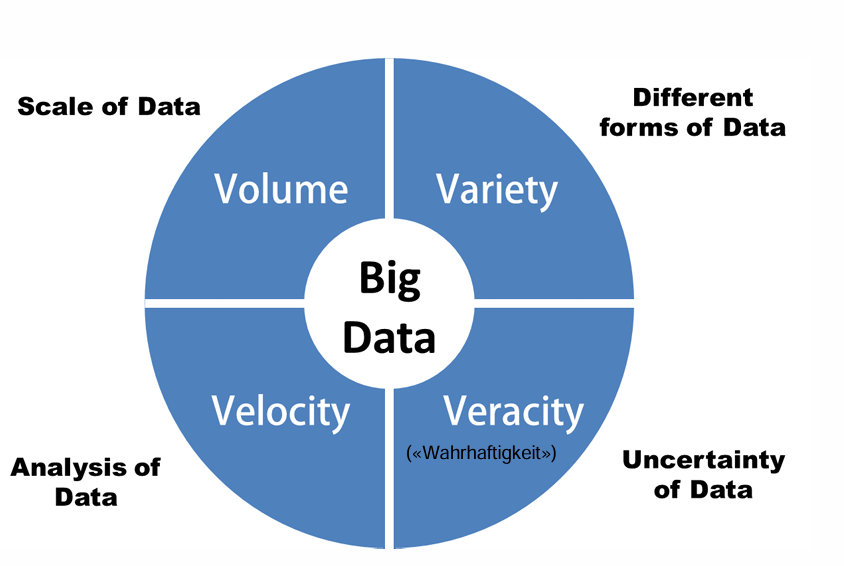
\includegraphics[width=0.75\linewidth]{Images/4v-bigdata.png}
    \caption{Die 4 V's von Big Data}
\end{figure}

\begin{figure}[H]
    \centering
    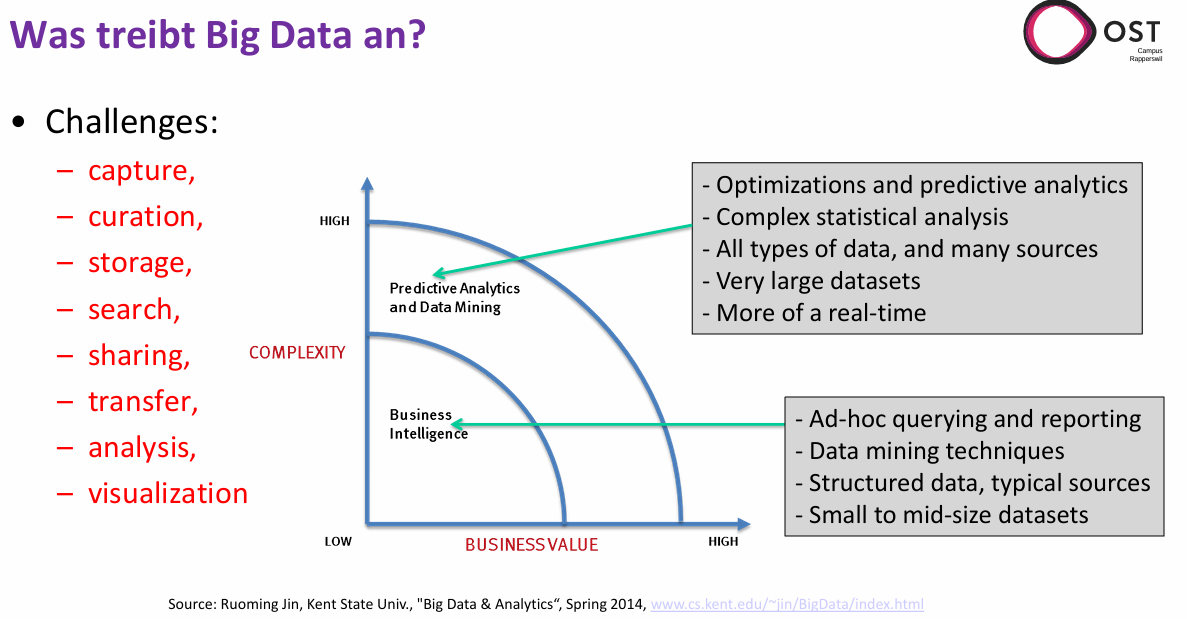
\includegraphics[width=1\linewidth]{Images/treiber-bigdata.png}
    \caption{Die Treiber von Big Data}
\end{figure}

\defn{Big Data Analytics}{
    Vielmals ist bei Big Data Analytics real-time analysen erforderlich.
    Dazu sind traditionelle Data Warehouse Architekuren ungeeignet.
    \begin{description}
        \item[Ansatz 1] Scaling Up, In-Memory Column Stores
        \item[Ansatz 2] Scaling Out, Shared Nothing Architektur, Verteilte Systeme  
    \end{description}
}

\begin{figure}[H]
    \centering
    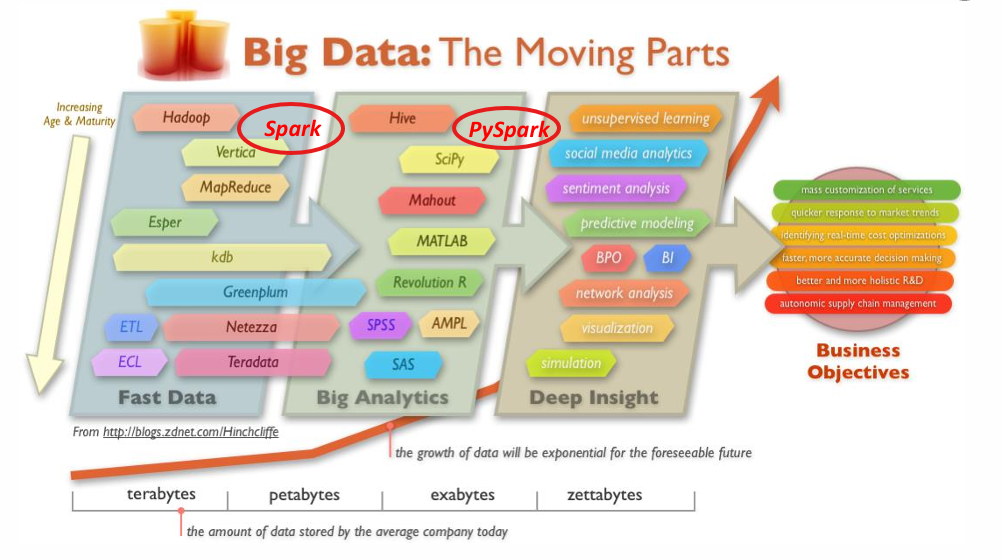
\includegraphics[width=0.75\linewidth]{Images/bigdata-tech.png}
    \caption{Big Data Technology Landscape}
\end{figure}

\section{Analytical Processing}
\defn{In-Memory Column Store}{
    \begin{itemize}
        \item \textbf{Column Store:} Spaltenorientiertes DMBS
            \begin{itemize}
                \item Bessere Komprimierung
                \item Bessere Indexierung
                \item Datenverwaltung pro Spalte
            \end{itemize}
        \item In-Memory:
            \begin{itemize}
                \item Nur Memory
                \item Keine Persistenz
                \item Persistenz durch logischem WAL oder Snapshots
            \end{itemize}
    \end{itemize}
    Bietet aufgrund der Architektur schnellere OLAP-Lese-Anfragen (10-100x)
    sind jedoch langsamer bei Updates und daher ungeeignet für write-heavy OLTP.
}

Produkte:
\begin{itemize}
    \item Oracle 12 (Erweiterung)
    \item MSSQL (Erweiterung)
    \item PostgreSQL (Third Party Erweiterung)
    \item SAP Hana (Standard, teuer, grosse Ressourcenanforderungen (Memory 500GB))
    \item Hbase
\end{itemize}

Weitere Optimierungen:
\begin{itemize}
    \item Materialisierte Strukturen
    \item Indexe
    \item Parallel Query Processing
    \item Vectorized Query Processing Style (Tupel Batches als Vektoren, SIMD) vs. Volcano (einzelne Tupel)
\end{itemize}

\section{Verteilte Technologien und Tools}
\subsection{Map-Reduce}
MapReduce war lange ein Kernkonzept in der Big-Data-Welt, insbesondere in Hadoop-Umgebungen.
Es ist noch in bestimmten Szenarien wichtig, wie z.B. Massive Batch-Jobs, Log
Analysen, verteilte Berechnungen ohne Echtzeitanforderungen.
Technologien wie Apache Spark, Dask, Vaex und Cloud-Data-Warehouses (z.B. 
BigQuery, Snowflake) sind inzwischen populärer.
\begin{itemize}
    \item Google
    \item Funktionales Modell gür gross angelegte Datenverarbeitung mittels vielen Computern
    \item Hohe Parallelität und Verfügbarkeit
    \item HDFS (Hadoop File System)
    \item Map-Reduce wird immer auf Disk geschrieben (langsamer als Spark)
    \item Hohe Abstraktion für den Benutzer (einfachere Handhabung)
\end{itemize}

\begin{figure}[H]
    \centering
    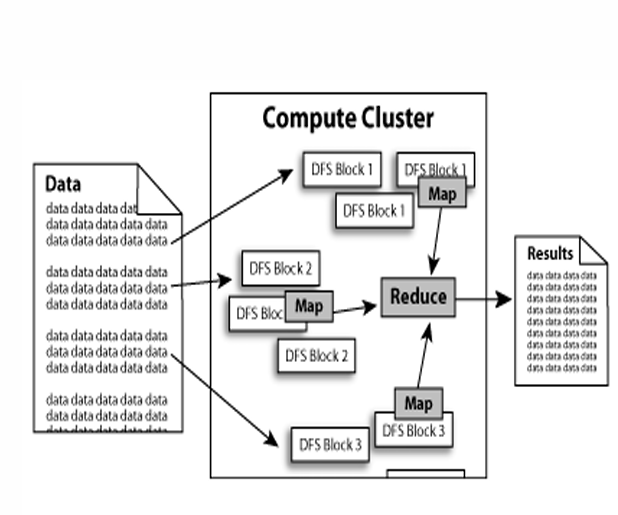
\includegraphics[width=0.5\linewidth]{Images/map-reduce.png}
    \caption{Map-Reduce Diagramm}
\end{figure}

Nachteile:
\begin{itemize}
    \item Master ist SPOF
    \item Master ist Engpass für Skalierbarkeit
    \item Latenz beim Öffnen von Dateien
\end{itemize}

\subsection{Spark}
Ist eine Open-Source (2010) Big-Data-Framework mit verteilter Architektur.
Benutzt schnelles In-Memory Computing.
Geschrieben in Scala mit Spark API für Python, Java, R und Clojure (Lisp)

\begin{figure}[H]
    \centering
    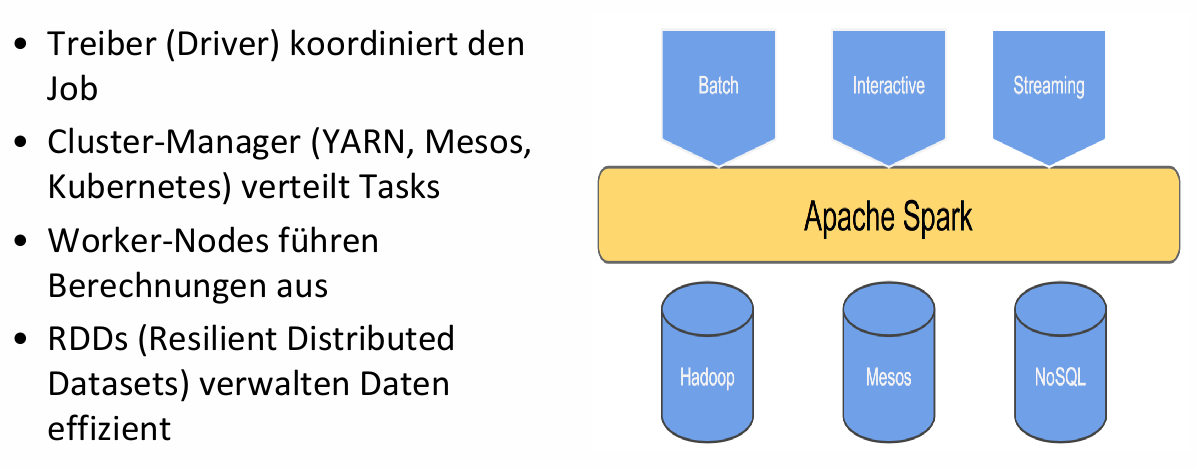
\includegraphics[width=1\linewidth]{Images/spark-architektur.png}
    \caption{Spark Architektur: Driver ist z.B der Benutzer via PySpark.
    Spark erstellt Abstraktionsebene auf Datenablage. 
    Beliebige Nodes können hinzugefügt werden (Horizontale Skalierung).}
\end{figure}
\begin{figure}[H]
    \centering
    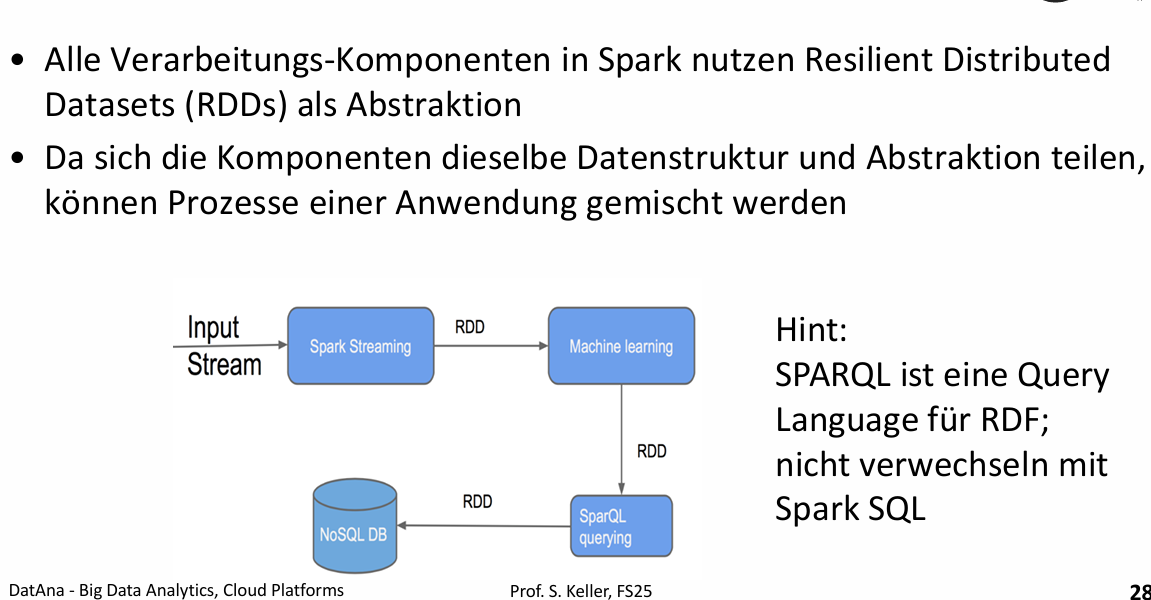
\includegraphics[width=1\linewidth]{Images/RDD.png}
    \caption{RDD's sind immutable und können nur als Input oder Output von Funktionen verwendet werden}
\end{figure}
\begin{figure}[H]
    \centering
    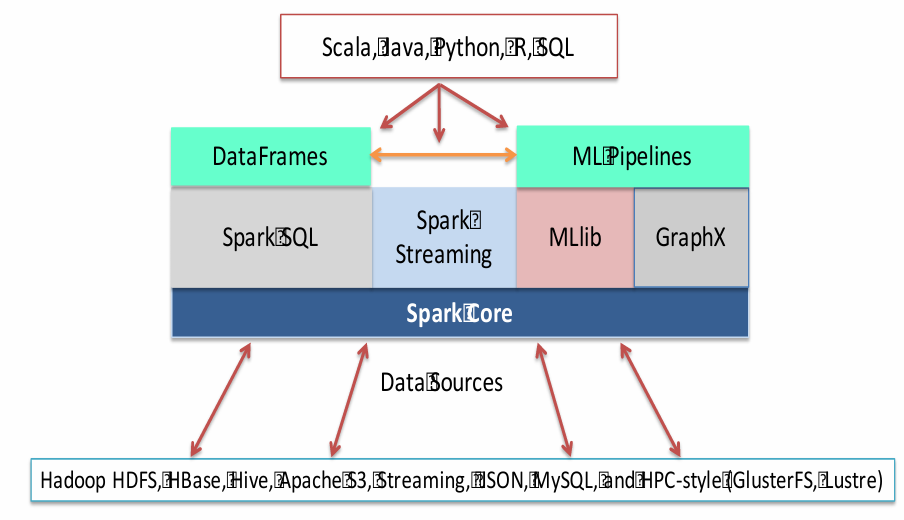
\includegraphics[width=1\linewidth]{Images/spark-ecosystem.png}
    \caption{Spark Ecosystem}
\end{figure}
\begin{figure}[H]
    \centering
    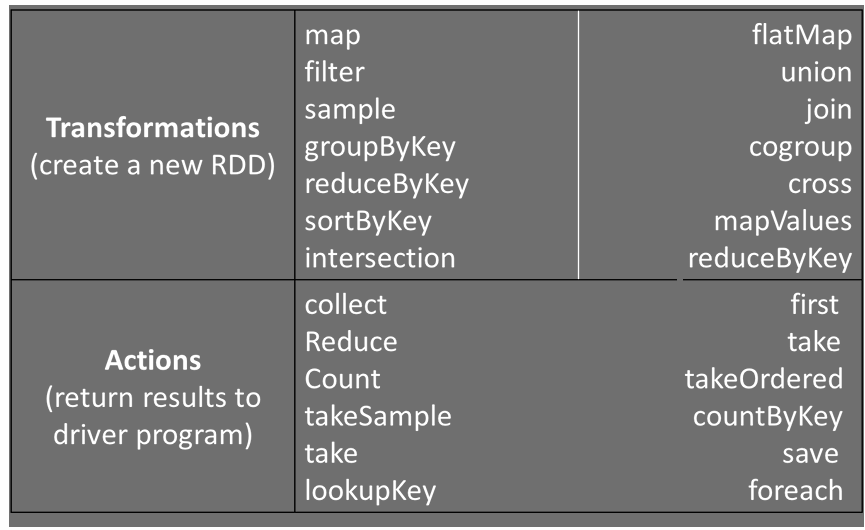
\includegraphics[width=1\linewidth]{Images/spark-operations.png}
    \caption{Spark Operations}
\end{figure}

Leistungsmerkmale:
\begin{itemize}
    \item Kann Daten vollkommen In-Memory verarbeiten (im Vergleich zu Map-Reduce)
    \item Wenn RDD nicht in Memory passt, verschlechtert sich die Performance
\end{itemize}

\subsection{Spark Notebook}

\begin{figure}[H]
    \centering
    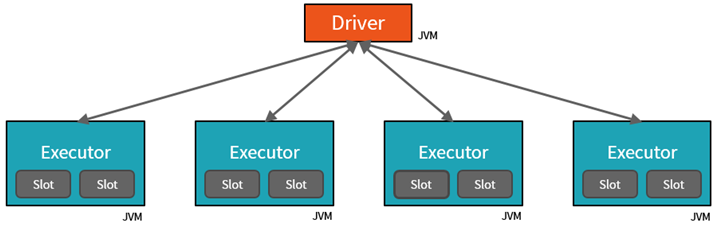
\includegraphics[width=1\linewidth]{Images/spark-driver.png}
    \caption{Spark Driver JVM}
\end{figure}
Jeder Executor hat eine Anzahl "Slots" (Apache Spark nennt diese "Cores", auch wenn sie nicht direkt mit 
den physischen CPU-Kernen zu tun haben). Das sind Threads, auf denen die eigentliche Rechenarbeit geschieht.
\begin{figure}[H]
    \centering
    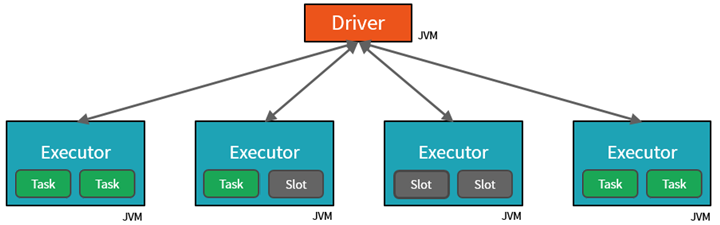
\includegraphics[width=1\linewidth]{Images/spark-driver-slot.png}
    \caption{Der "Driver" schickt Aufgaben (Tasks) an die leeren Slots der Executors, um Arbeit aufzuteilen}
\end{figure}

\begin{lstlisting}[language=Python]
# DF API is similar to pandas API
fire_service_calls_df = spark.read.csv(
        SF_FIRE_CALL_CSV_URL, header=True, schema=fire_schema
    )
# Column Names
fire_service_calls_df.columns

# Row Count
fire_service_calls_df.count()
# -> 6 892 945
\end{lstlisting}
\begin{figure}[H]
    \centering
    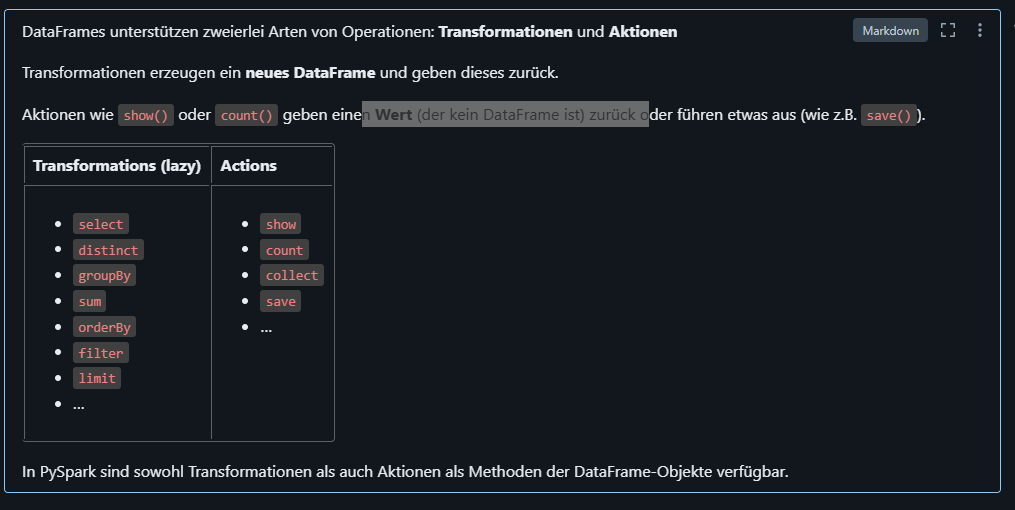
\includegraphics[width=1\linewidth]{Images/spark-df-actions.png}
    \caption{Spark Aktionen auf oder an DF}
\end{figure}
Im Gegensatz zu Transformationen auf Pandas-DataFrames wird beim Aufruf
von Spark-DataFrame-Transformationen noch nichts "wirklich" ausgeführt,
sondern nur die Transformation im Query-Plan des zurückgegebenen neuen DataFrames vermerkt.

Erst beim Aufruf einer Aktion wird der Query-Plan (mit allen so angesammelten Transformationen und mit der Aktion)
optimiert und dann ausgeführt.

\begin{lstlisting}[language=Python]
# select distinct call types
fire_service_calls_df.select('CallType').distinct().show()


# count distinct call types
fire_service_calls_df.select('CallType').distinct().count()
\end{lstlisting}

\begin{lstlisting}[language=Python]
# register new sql context on df for sql queries
sqlContext.registerDataFrameAsTable(
        fire_service_calls_df, "fireServiceCalls"
    )

# query via sql
# %sql ist eine Databricks-spezifische "Notebook Magic", 
# die in Jupyter (oder in Python-Programmen, die Spark als 
# Bibliothek verwenden) nicht zur Verfuegung steht.
%sql
SELECT CallType
FROM fire_service_calls_df
LIMIT 5;

# Oder via Python
spark.sql(
  """
  SELECT CallType
  FROM fireServiceCalls
  LIMIT 5
  """
).show()
\end{lstlisting}


\begin{lstlisting}[language=Python]
# schema ausgeben
fire_service_calls_df.printSchema()

from pyspark.sql.functions import year
# Wieviele Jahre umfassen die vorliegenden Notrufdaten?
fire_service_calls_ts_df
    .select(year('CallDateTS'))
    .distinct()
    .orderBy('year(CallDateTs)')
    .show()

# Bis zu welchem Datum gehen die Daten?
fire_service_calls_ts_df
    .agg({"CallDateTS": "max"})
    .collect()

# Anruf Zahl pro Tag
count_df = fire_service_calls_ts_df \
  .filter('CallDateTS >= "2015-06-28"') \
  .filter('CallDateTS <= "2015-07-10"') \
  .groupBy('CallDateTS') \
  .count() \
  .orderBy('CallDateTS')

count_df.show()

# Gibt die Anzahl Paritionen zurueck
# in welche die Daten verteilt werden
fire_service_calls_df.rdd.getNumPartitions()

# Neupartitionierung
fire_service_calls_ts_8partitions_df = 
    fire_service_calls_ts_df.repartition(8)
\end{lstlisting}
Wenn ein Job sich auf mehrere Tasks aufteilen lässt, bearbeitet jeder Task eine dieser Partitions.
Die Tasks werden auf zur Ausführung auf die Executor-Slots verteilt und die Ergebnisse dann zusammengeführt.
Bei der Ausführung können Tasks, die gleichzeitig in verschiedenen Slots liegen, parallel ausgeführt werden.

\end{document}
